%% ============================================================
%% DOCUMENT CLASS
%% ============================================================
\documentclass{article}
\usepackage[table,dvipsnames]{xcolor}

%% ============================================================
%% EMBEDDED BIBLIOGRAPHY
%% ============================================================
\begin{filecontents*}{refs.bib}
@techreport{bis2017,
  author       = {{Basel Committee on Banking Supervision}},
  title        = {Basel {III}: Finalising Post-Crisis Reforms},
  institution  = {Bank for International Settlements},
  year         = {2017},
  url          = {https://www.bis.org/bcbs/publ/d424.pdf}
}
@techreport{sec2019,
  author       = {{Securities and Exchange Commission}},
  title        = {Regulation Best Interest: The Broker-Dealer Standard of Conduct},
  institution  = {U.S. Securities and Exchange Commission},
  year         = {2019},
  number       = {Release No.\ 34-86031},
  url          = {https://www.sec.gov/rules/final/2019/34-86031.pdf}
}
@techreport{gdpr2016,
  author       = {{European Parliament and Council of the European Union}},
  title        = {Regulation ({EU}) 2016/679 on the Protection of Natural
                  Persons with Regard to the Processing of Personal Data ({GDPR})},
  institution  = {Official Journal of the European Union},
  year         = {2016},
  url          = {https://eur-lex.europa.eu/legal-content/EN/TXT/PDF/?uri=CELEX:32016R0679}
}
@article{governatore2005,
  author  = {G. Governatori and Z. Milosevic and S. Sadiq},
  title   = {Compliance Checking Between Business Processes and Business Contracts},
  journal = {Proceedings of the 10th International Enterprise Distributed
             Object Computing Conference},
  year    = {2005},
  pages   = {221--232},
  doi     = {10.1109/EDOC.2006.2}
}
@article{chalkidis2020,
  author  = {I. Chalkidis and M. Fergadiotis and P. Malakasiotis
             and N. Aletras and I. Androutsopoulos},
  title   = {{LEGAL-BERT}: The Muppets Straight Out of Law School},
  journal = {Findings of the Association for Computational Linguistics: EMNLP 2020},
  year    = {2020},
  pages   = {2898--2904},
  doi     = {10.18653/v1/2020.findings-emnlp.261}
}
@article{cao2024,
  author  = {Z. Cao and Z. Feinstein},
  title   = {Large Language Models in Financial Regulatory Interpretation},
  journal = {arXiv preprint},
  year    = {2024},
  volume  = {arXiv:2309.04175}
}
@article{pan2024,
  author  = {S. Pan and L. Luo and Y. Wang and C. Chen and J. Wang and X. Wu},
  title   = {Unifying Large Language Models and Knowledge Graphs: A Roadmap},
  journal = {IEEE Transactions on Knowledge and Data Engineering},
  year    = {2024},
  volume  = {36},
  number  = {7},
  pages   = {3580--3599},
  doi     = {10.1109/TKDE.2024.3352100}
}
@article{karma2025,
  author  = {Y. Lu and J. Wang},
  title   = {{KARMA}: Leveraging Multi-Agent {LLMs} for Automated
             Knowledge Graph Enrichment},
  journal = {arXiv preprint},
  year    = {2025},
  volume  = {arXiv:2502.06472}
}
@article{graphrag2024,
  author  = {D. Edge and H. Trinh and N. Cheng and J. Bradley
             and A. Chao and A. Mody and S. Truitt and J. Larson},
  title   = {From Local to Global: A {GraphRAG} Approach to
             Query-Focused Summarization},
  journal = {arXiv preprint},
  year    = {2024},
  volume  = {arXiv:2404.16130}
}
@article{bloomberggpt2023,
  author  = {S. Wu and O. Irsoy and S. Lu and V. Dabravolski
             and M. Dredze and S. Gehrmann and P. Kambadur
             and D. Rosenberg and G. Mann},
  title   = {{BloombergGPT}: A Large Language Model for Finance},
  journal = {arXiv preprint},
  year    = {2023},
  volume  = {arXiv:2303.17564}
}
@article{finbert2020,
  author  = {Y. Yang and M. C. S. Uy and A. Huang},
  title   = {{FinBERT}: A Pretrained Language Model for Financial Communications},
  journal = {arXiv preprint},
  year    = {2020},
  volume  = {arXiv:2006.08097}
}
@article{lisurvey2024,
  author  = {Y. Li and Z. Wang and B. Ding and L. Li and Y. Li and Q. Liao},
  title   = {Large Language Models in Finance: A Survey},
  journal = {Proceedings of the 4th {ACM} International Conference on {AI} in Finance},
  year    = {2024},
  pages   = {374--382},
  doi     = {10.1145/3604237.3626869}
}
@article{maynez2020,
  author  = {J. Maynez and S. Narayan and B. Bohnet and R. McDonald},
  title   = {On Faithfulness and Factuality in Abstractive Summarization},
  journal = {Proceedings of the 58th Annual Meeting of the
             Association for Computational Linguistics},
  year    = {2020},
  pages   = {1906--1919},
  doi     = {10.18653/v1/2020.acl-main.173}
}
@article{singhal2023,
  author  = {K. Singhal and S. Azizi and T. Tu and S. S. Mahdavi
             and J. Wei and H. W. Chung and N. Scales and A. Tanwani
             and H. Cole-Lewis and S. Pfohl},
  title   = {Large Language Models Encode Clinical Knowledge},
  journal = {Nature},
  year    = {2023},
  volume  = {620},
  pages   = {172--180},
  doi     = {10.1038/s41586-023-06291-2}
}
@article{dahl2024,
  author  = {M. Dahl and V. Magesh and M. Suzgun and D. Ho},
  title   = {Large Legal Fictions: Profiling Legal Hallucinations in Large Language Models},
  journal = {Journal of Legal Analysis},
  year    = {2024},
  volume  = {16},
  number  = {1},
  pages   = {64--93},
  doi     = {10.1093/jla/laae003}
}
@article{openai2024,
  author  = {{OpenAI}},
  title   = {{GPT-4} Technical Report},
  journal = {arXiv preprint},
  year    = {2024},
  volume  = {arXiv:2303.08774}
}
@techreport{anthropic2024,
  author      = {{Anthropic}},
  title       = {The {Claude 3} Model Family: {Opus, Sonnet, Haiku}
                  -- Model Card},
  institution = {Anthropic},
  year        = {2024},
  month       = {3},
  url         = {https://www-cdn.anthropic.com/de8ba9b01c9ab7cbabf5c33b80b7bbc618857627/Model_Card_Claude_3.pdf}
}
@article{llama2024,
  author  = {A. Dubey and A. Jauhri and A. Pandey and A. Kadian and others},
  title   = {The {Llama 3} Herd of Models},
  journal = {arXiv preprint},
  year    = {2024},
  volume  = {arXiv:2407.21783}
}
@misc{qwen2024,
  author       = {{Qwen Team}},
  title        = {{Qwen3}: Technical Report},
  year         = {2024},
  howpublished = {\url{https://qwenlm.github.io/blog/qwen3/}},
  note         = {Mixture-of-Experts model series; Qwen3-235B-A22B-Instruct used here}
}
@article{reimers2019,
  author  = {N. Reimers and I. Gurevych},
  title   = {Sentence-{BERT}: Sentence Embeddings Using Siamese {BERT}-Networks},
  journal = {Proceedings of the 2019 Conference on Empirical Methods
             in Natural Language Processing},
  year    = {2019},
  pages   = {3982--3992},
  doi     = {10.18653/v1/D19-1410}
}
@article{networkx2008,
  author    = {A. A. Hagberg and D. A. Schult and P. J. Swart},
  title     = {Exploring Network Structure, Dynamics, and Function Using {NetworkX}},
  booktitle = {Proceedings of the 7th {Python} in Science Conference},
  year      = {2008},
  pages     = {11--15}
}
@misc{rigcode2025,
  author = {{Vikash Kumar}},
  title  = {{RIG} Pipeline: Regulatory Intent Graph for {LLM}-Assisted Compliance Extraction},
  year   = {2025},
  url    = {https://github.com/vksabnima/rig_pipeline},
  note   = {MIT License}
}
\end{filecontents*}

%% ============================================================
%% PACKAGES
%% ============================================================
\usepackage[utf8]{inputenc}
\usepackage{authblk}
\usepackage{setspace}
\usepackage[margin=1.25in]{geometry}
\usepackage{graphicx}
\graphicspath{ {./figures/} }
\usepackage{subcaption}
\usepackage{amsmath}
\usepackage{amssymb}
\usepackage{lineno}
\usepackage{hyperref}
\usepackage{booktabs}
\usepackage{multirow}
\usepackage{array}
\usepackage{tikz}
\usepackage{pgfplots}
\usepackage{pgfplotstable}
\pgfplotsset{compat=1.18}
\usetikzlibrary{shapes.geometric,arrows.meta,positioning,
                fit,backgrounds,calc,matrix,decorations.pathreplacing}
\usepackage[style=nejm,citestyle=numeric-comp,sorting=none]{biblatex}
\addbibresource{refs.bib}

\title{RIG: A Regulatory Intent Graph Methodology for LLM-Assisted
Compliance Extraction from Financial Documents}

\author[1*]{Vikash Kumar}
\affil[1]{Independent Researcher, Austin, Texas, USA.}
\affil[*]{Address correspondence to: vikash.singh261@gmail.com}
\date{}
\onehalfspacing

\definecolor{navyblue}{RGB}{31,73,125}
\definecolor{steelblue}{RGB}{70,130,180}
\definecolor{lightblue}{RGB}{173,216,230}
\definecolor{burntorange}{RGB}{204,85,0}
\definecolor{forestgreen}{RGB}{34,139,34}
\definecolor{lightgray}{RGB}{220,220,220}
\definecolor{darkgray}{RGB}{80,80,80}
\definecolor{cellhigh}{RGB}{8,69,148}
\definecolor{cellmid}{RGB}{107,174,214}
\definecolor{celllow}{RGB}{247,251,255}

\begin{document}
\begin{nolinenumbers}
\maketitle
\end{nolinenumbers}
\linenumbers

%% ================================================================
%%  ABSTRACT
%% ================================================================
\begin{abstract}
Financial regulatory compliance requires precise extraction of
structured obligations from dense legal text, a task prone to human
error and difficult to scale. We introduce the Regulatory Intent
Graph (RIG), a five-stage LLM pipeline that segments regulatory text
into atomic obligation clauses, extracts structured six-field
tuples, and constructs queryable knowledge graphs. Applied to 2{,}167
obligation clauses from Basel~III, SEC Regulation Best Interest, and
the EU~GDPR, RIG produces a cross-jurisdictional Unified Compliance
Graph of 4{,}603 nodes, 74{,}306 edges, and 2{,}390 cross-document
obligation alignments. We define five evaluation metrics---RCC, OAL,
RIF, CAS, and HRR---with HRR decomposed into detection and stability
sub-components. Multi-model benchmarking across four LLMs (GPT-4o,
Claude~Sonnet, Qwen3-235B, Llama-3-8B) yields three findings: (i)
Claude~Sonnet achieves statistically significantly higher RIF than
GPT-4o on both human-annotated documents (non-overlapping 95\%
bootstrap CIs); (ii) among frontier-class extractors, above-threshold
cross-document alignment precision is near-invariant (CAS range
0.003); (iii) the smaller dense open model achieves the highest raw
coverage (RCC 0.998) and attribute fill (OAL 0.820) yet the lowest
Reg~BI fidelity (0.364), revealing \emph{template-following
inflation}---aggressively uniform outputs that inflate OAL and
composite HRR without gold-aligned fidelity. GDPR yields the highest
per-model OAL (0.735--0.803), confirming that OAL captures structural
differences in regulatory drafting. Error analysis of the 30
lowest-fidelity GPT-4o extractions shows that cross-reference
dependencies drive 90\% of failures, identifying a tractable
architectural target for future work.
\end{abstract}

%% ================================================================
%%  1. INTRODUCTION
%% ================================================================
\section{INTRODUCTION}

Financial institutions operate under regulatory frameworks of extraordinary
and growing complexity.
The Basel~III capital adequacy framework spans 161~pages and encodes
hundreds of distinct obligations governing risk weights, capital buffers,
and supervisory expectations~\cite{bis2017}.
The SEC Regulation Best Interest (Reg~BI), governing broker-dealer conduct
standards, spans 770~pages with 911~extractable obligation
clauses~\cite{sec2019}.
The EU General Data Protection Regulation (GDPR), applicable to any
organization handling personal data of EU residents, contributes a further
498~structured obligations~\cite{gdpr2016}.
Together these three frameworks encode 2,167~distinct compliance obligations
across 1,019~pages of dense legal prose---and they represent only a small
fraction of the global regulatory landscape.

Compliance officers and regulatory technology (RegTech) teams must track
these obligations across documents, identify inter-framework dependencies,
detect potential conflicts, and verify implementation coverage---tasks
routinely performed through manual review at significant cost and with
non-trivial error rates.
The rise of large language models (LLMs) offers a compelling path toward
automating this process, yet the field lacks rigorous evaluation frameworks,
validated metrics, and reproducible benchmark results.
Existing work either applies LLMs to regulatory question-answering
tasks~\cite{cao2024} or constructs general-purpose legal knowledge
graphs~\cite{pan2024} without addressing the specific demands of
multi-framework compliance obligation extraction: structured tuple fidelity,
cross-document dependency discovery, and adversarial robustness under
regulatory text perturbation.

We address this gap with three principal contributions.
First, we introduce the \textbf{Regulatory Intent Graph (RIG)}, a
five-stage pipeline that segments regulatory text into atomic obligation
clauses, extracts structured six-field tuples
$\langle$\textit{subject, obligation, condition, threshold, deadline,
exception}$\rangle$ via LLM inference, and constructs directed knowledge
graphs encoding obligation dependencies.
Second, we introduce \textbf{five evaluation metrics}---RCC, OAL,
RIF, CAS, and HRR---designed specifically for regulatory extraction
evaluation, with a decomposition of HRR into detection and stability
sub-components that reveals an extraction-robustness tradeoff not
previously reported.
Third, we produce the first \textbf{cross-jurisdictional Unified Compliance
Graph (UCG)}, to our knowledge, merging obligation graphs from three distinct regulatory
regimes to surface 2,390 cross-document obligation alignments invisible to
single-document analysis.

Empirical evaluation across GPT-4o, Claude~Sonnet, Qwen3-235B, and
Llama-3-8B establishes three principal findings: (i) all four models
achieve near-complete extraction coverage (RCC~$>$~0.90), with
statistically significant pairwise RIF differences between models on
the gold-validated subset; (ii) among the three frontier-class models,
above-threshold cross-document alignment precision is near-invariant
(CAS range 0.003) under a fixed sentence-embedding and threshold,
making similarity-based alignment robust to frontier-extractor choice;
and (iii) the smaller dense open model (Llama-3-8B) exhibits
\textit{template-following inflation}---aggressively uniform
extractions that jointly inflate OAL, CAS, and HRR-Stability while
suppressing gold-aligned RIF---demonstrating that composite robustness
and richness scores require decomposition against gold fidelity.
Taken together, these findings provide the first rigorous empirical
characterization of LLM capabilities and limitations for
production-scale financial regulatory compliance extraction.

%% ================================================================
%%  2. RELATED WORK
%% ================================================================
\section{RELATED WORK}

\textbf{NLP for regulatory and legal text.}
Early efforts to automate regulatory analysis relied on rule-based
systems and deontic logic frameworks~\cite{governatore2005}.
Transformer-based models enabled advances in legal document understanding,
with domain-adapted models such as Legal-BERT~\cite{chalkidis2020}
achieving strong performance on legal classification tasks.
Recent work has applied LLMs specifically to financial regulation:
Cao and Feinstein~\cite{cao2024} demonstrated LLM utility for regulatory
interpretation tasks.
Our work extends this line by addressing multi-document,
cross-jurisdiction extraction with structured tuple output, validated
metrics, and adversarial evaluation---capabilities absent from prior
benchmarks.

\textbf{LLMs and knowledge graph construction.}
Pan~et~al.~\cite{pan2024} survey LLM--knowledge graph integration,
identifying structured extraction and graph alignment as open challenges.
The KARMA framework~\cite{karma2025} employs multi-agent LLM pipelines
for knowledge graph enrichment in scientific domains.
GraphRAG~\cite{graphrag2024} constructs community-level summaries from
document graphs for retrieval augmentation.
Our work addresses a complementary problem: constructing obligation-typed
graphs where node semantics are legally defined and edge semantics
are structurally critical for compliance verification.

\textbf{Financial AI and RegTech.}
BloombergGPT~\cite{bloomberggpt2023} and FinBERT~\cite{finbert2020}
demonstrated the value of domain-specific pretraining for financial NLP.
Recent surveys~\cite{lisurvey2024} cover LLM applications in finance
including risk modeling, fraud detection, and regulatory interpretation.
No prior work, however, addresses structured obligation extraction with
cross-document alignment or provides adversarial robustness evaluation
on financial regulatory text.

\textbf{Adversarial robustness of LLMs.}
Hallucination in LLMs is well-documented~\cite{maynez2020}, with
particular concerns in high-stakes domains such as
medicine~\cite{singhal2023} and law~\cite{dahl2024}.
Prior adversarial evaluation frameworks focus primarily on factual recall.
Our HRR decomposition introduces adversarial evaluation specific to
structured extraction, distinguishing detection of non-obligation text
from stability under obligation-preserving perturbations, and revealing
that these two properties are independently distributed across models.

%% ================================================================
%%  3. METHODS
%% ================================================================
\section{METHODS}

\subsection{Experimental and Technical Design}

Figure~\ref{fig:pipeline} illustrates the complete RIG pipeline.
Raw regulatory PDFs are processed through five sequential stages:
clause segmentation, structured tuple extraction, graph construction,
cross-document alignment, and metric computation.
All stages are implemented in Python using publicly available libraries;
the full pipeline is reproducible via the accompanying
repository~\cite{rigcode2025}.

\begin{figure}[!htbp]
\centering
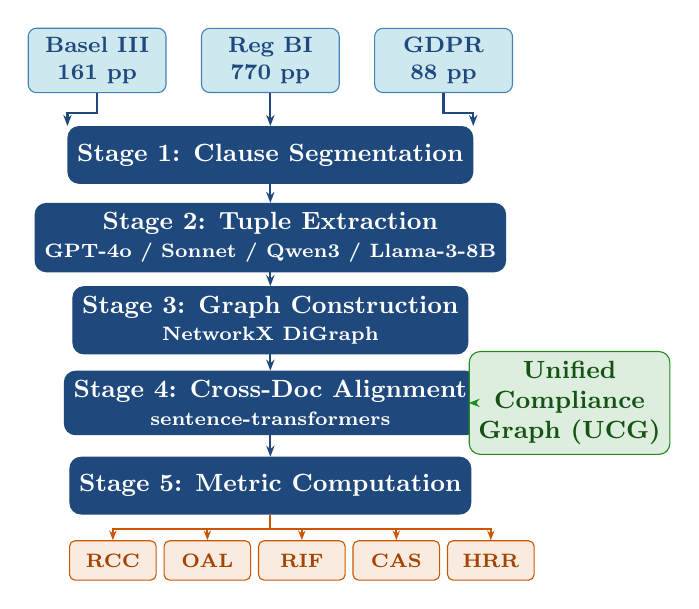
\begin{tikzpicture}[
  box/.style={rectangle, rounded corners=4pt,
    draw=navyblue, fill=navyblue, text=white,
    minimum width=2.8cm, minimum height=0.72cm,
    font=\small\bfseries, align=center},
  docbox/.style={rectangle, rounded corners=3pt,
    draw=steelblue, fill=lightblue!60, text=navyblue,
    minimum width=1.75cm, minimum height=0.58cm,
    font=\footnotesize\bfseries, align=center},
  outbox/.style={rectangle, rounded corners=4pt,
    draw=forestgreen, fill=forestgreen!15, text=forestgreen!60!black,
    minimum width=2.4cm, minimum height=0.72cm,
    font=\small\bfseries, align=center},
  metbox/.style={rectangle, rounded corners=2pt,
    draw=burntorange, fill=burntorange!12, text=burntorange!80!black,
    minimum width=1.1cm, minimum height=0.50cm,
    font=\scriptsize\bfseries, align=center},
  arr/.style={-{Stealth[length=4pt]}, thick, navyblue},
  oarr/.style={-{Stealth[length=3.5pt]}, thick, burntorange}
]
\node[docbox] (b3)   at (0, 0)    {Basel~III\\161~pp};
\node[docbox] (rbi)  at (2.2,0)   {Reg~BI\\770~pp};
\node[docbox] (gdpr) at (4.4,0)   {GDPR\\88~pp};
\node[box] (s1) at (2.2,-1.2)  {Stage 1: Clause Segmentation};
\node[box] (s2) at (2.2,-2.25) {Stage 2: Tuple Extraction\\[-1pt]{\scriptsize GPT-4o / Sonnet / Qwen3 / Llama-3-8B}};
\node[box] (s3) at (2.2,-3.30) {Stage 3: Graph Construction\\[-1pt]{\scriptsize NetworkX DiGraph}};
\node[box] (s4) at (2.2,-4.35) {Stage 4: Cross-Doc Alignment\\[-1pt]{\scriptsize sentence-transformers}};
\node[box] (s5) at (2.2,-5.40) {Stage 5: Metric Computation};
\draw[arr] (b3.south)   -- ++(0,-.25) -| (s1.north west);
\draw[arr] (rbi.south)  -- (s1.north);
\draw[arr] (gdpr.south) -- ++(0,-.25) -| (s1.north east);
\draw[arr] (s1)--(s2); \draw[arr] (s2)--(s3);
\draw[arr] (s3)--(s4); \draw[arr] (s4)--(s5);
\node[outbox] (ucg) at (6.0,-4.35) {Unified\\Compliance\\Graph (UCG)};
\draw[arr,forestgreen] (s4.east) -- (ucg.west);
\node[metbox] (rcc) at (0.2,-6.35)  {RCC};
\node[metbox] (oal) at (1.4,-6.35)  {OAL};
\node[metbox] (rif) at (2.6,-6.35)  {RIF};
\node[metbox] (cas) at (3.8,-6.35)  {CAS};
\node[metbox] (hrr) at (5.0,-6.35)  {HRR};
\foreach \m in {rcc,oal,rif,cas,hrr}
  \draw[oarr] (s5.south) -- ++(0,-.18) -| (\m.north);
\end{tikzpicture}
\caption{\textbf{RIG pipeline architecture.}
Three regulatory PDFs from distinct jurisdictions enter a five-stage
pipeline producing per-document knowledge graphs, a cross-jurisdictional
Unified Compliance Graph (UCG), and five evaluation metrics.}
\label{fig:pipeline}
\end{figure}

\subsection{Stage 1: Clause Segmentation}

Each regulatory PDF is parsed using \texttt{pdfplumber} with custom
post-processing to remove headers, footers, and footnote markers.
A rule-based segmenter classifies each sentence into one of four types
based on regulatory signal words: \textsc{Obligation} (``shall'',
``must'', ``required to''), \textsc{Condition} (``if'', ``where'',
``when''), \textsc{Exception} (``unless'', ``except'', ``provided
that''), and \textsc{Declarative} (all other).
Only \textsc{Obligation} and \textsc{Condition} clauses are forwarded
to extraction.
This segmentation produced 758, 911, and 498 obligation clauses from
Basel~III, Reg~BI, and GDPR respectively (Table~\ref{tab:corpus}).

\begin{table}[!htbp]
\caption{Regulatory document corpus statistics.}
\centering
\begin{tabular}{lrrrr}
\toprule
Document & Pages & Clauses & Graph Nodes & Graph Edges \\
\midrule
Basel III~\cite{bis2017}  & 161   & \phantom{0,}758 & 1,624 & 29,339 \\
SEC Reg BI~\cite{sec2019} & 770   & \phantom{0,}911 & 1,798 & 41,052 \\
EU GDPR~\cite{gdpr2016}   & \phantom{0}88 & \phantom{0,}498 & 1,181 & \phantom{0}3,915 \\
\midrule
\textbf{Total} & \textbf{1,019} & \textbf{2,167} & \textbf{4,603} & \textbf{74,306} \\
\bottomrule
\end{tabular}
\label{tab:corpus}
\end{table}

\subsection{Stage 2: Structured Tuple Extraction}

For each segmented obligation clause, we prompt each LLM with a
zero-shot instruction requesting a structured six-field JSON tuple:
\begin{equation}
T = \langle\, s,\; o,\; c,\; \theta,\; d,\; e \,\rangle
\end{equation}
where $s$ is the regulated \textit{subject}, $o$ is the
\textit{obligation} statement, $c$ is the triggering \textit{condition},
$\theta$ is a numeric or categorical \textit{threshold}, $d$ is a
\textit{deadline}, and $e$ is an \textit{exception}.
Fields not present in the source clause are returned as JSON \texttt{null}.
Four models are evaluated: GPT-4o~\cite{openai2024},
Claude~Sonnet~\cite{anthropic2024}, Qwen3-235B-A22B-Instruct
(open-weights Mixture-of-Experts model, 22B active parameters)
~\cite{qwen2024}, and Llama-3-8B-Instruct-Lite
(dense 8B-parameter open-weights model, INT4-quantized Together.ai
variant)~\cite{llama2024}.
All four models are accessed via hosted inference endpoints: closed
models through their respective vendor APIs, both open-weights models
through Together.ai's serverless infrastructure, with identical
prompt templates, temperature = 0, and fixed random seed for
reproducibility.

\subsection{Stage 3: Knowledge Graph Construction}

Extracted tuples are encoded as nodes in a directed graph $G=(V,E)$
using NetworkX~\cite{networkx2008}.
Three edge types are defined: \textsc{Triggers}
($c_j \rightarrow o_i$, where condition $c_j$ activates obligation
$o_i$), \textsc{DependsOn} ($o_i \rightarrow o_j$, detected via shared
subject and threshold cross-references), and \textsc{ExceptionOf}
($e_k \rightarrow o_i$).

\subsection{Stage 4: Cross-Document Alignment}

To construct the UCG, we embed each obligation node's associated text
using the \texttt{all-MiniLM-L6-v2} sentence-transformer~\cite{reimers2019}
and compute pairwise cosine similarity across all node pairs from
different source documents.
Pairs with cosine similarity $\geq \tau$ are retained as candidate
alignments.
The selected threshold $\tau=0.50$ is justified by the sensitivity
analysis in Section~\ref{sec:results}.
Two text-source conventions exist in the implementation: the root
cross-document alignment (Table~\ref{tab:ucg}) uses the full segmented
clause text preferentially; the per-model alignment used in
Table~\ref{tab:fullresults} uses the model's extracted obligation
description preferentially. This distinction is reconciled in the
captions of the two tables.

Stage 5 (metric computation) is described in
Section~\ref{sec:metrics}.

\subsection{Adversarial Robustness Evaluation}
\label{sec:adversarial_eval}

Two adversarial samples are drawn from the pooled Basel~III and Reg~BI
extraction outputs using \texttt{random.seed(42)}:
\textit{(i)} a 20-clause sample paired with all five perturbation
types for HRR-Stability, and \textit{(ii)} a 20-clause sample
paired with three of the five types (synonym swap, negation injection,
threshold mutation) for the composite HRR computation described in
Section~\ref{sec:metrics}.
Perturbations not producing any surface-level change are excluded,
yielding an effective perturbation count per model in the
range~57--69 (Table~\ref{tab:fullresults}).
The five perturbation types are synonym substitution
(\textit{semantic-preserving}), clause reordering
(\textit{semantic-preserving}), negation injection
(\textit{semantic-altering}), threshold mutation
(\textit{semantic-altering}), and entity substitution
(\textit{semantic-altering}).
Additionally, 15~\textit{hallucination bait} clauses were hand-crafted as
declarative statements that superficially resemble obligations but
contain no actionable requirement (e.g., ``The Basel Committee on Banking
Supervision was established in 1974 by the central bank governors of
the Group of Ten countries'').
Sample sizes are a deliberate scoping choice to limit live-API cost
during the benchmark run; scaling to the full 2,167-clause corpus is
straightforward and noted as future work.

\subsection{Gold Standard Annotation and Validation}

A gold standard of 758 clauses (Basel~III) was produced by a two-stage
process.
An automated pre-annotation pass using Claude~Sonnet generated initial
tuple labels for each clause.
All 758~rows were then validated by a second Claude~Sonnet pass acting
as an annotation validator, with explicit per-field confidence scoring,
yielding 449~accepted annotations (59.2\%) and 309~corrections (40.8\%)
at mean validator confidence~0.909.
The most frequently corrected field was \textit{subject\_gt}
(141~corrections; 45.6\% of all corrections), indicating that automated
annotation systematically struggles with regulated entity attribution
even when obligation content is correctly extracted.
The validated annotation set is used as ground truth for RIF
computation on Basel~III.
Reg~BI RIF values reported in Table~\ref{tab:fullresults} use this same
Basel~III gold set through an implementation keyed on clause identifiers
(\texttt{OBL-nnnn}) that overlap between documents; the resulting
Reg~BI RIF should be read as a gold-constrained lower bound and is
discussed in Section~\ref{sec:discussion}.
GDPR RIF uses a 50-clause GDPR gold set auto-annotated by Claude~Sonnet
and retained without additional human review.

To assess agreement between the LLM-based gold standard and an
independent human judgment, an independent human annotation pass
was conducted on a 100-clause stratified random sample of Basel~III
(short / medium / long buckets, $n \approx 33$ per bucket) without
prior exposure to the Claude annotations. Cohen's $\kappa$ is
computed per six-tuple field on a binary present/absent judgment;
content alignment when both raters mark a field present is reported
separately. Aggregate values across all 600 field judgments are
reported in Table~\ref{tab:kappa}; the worksheet and scoring script
are released with the code repository~\cite{rigcode2025}.

%% ================================================================
%%  4. EVALUATION METRICS
%% ================================================================
\section{EVALUATION METRICS}
\label{sec:metrics}

We define five metrics for regulatory extraction evaluation.
All metrics are computed per document--model pair unless stated otherwise.
Each equation below describes the exact formula implemented by the
experimental pipeline used to produce Table~\ref{tab:fullresults}.

\textbf{Regulatory Clause Coverage (RCC)}
measures the fraction of segmented obligation clauses for which a
model produces a tuple with at least one non-null field:
\begin{equation}
\text{RCC} = \min\!\left(\frac{|\{c_i \in C :
  \exists\, f \in F,\, T_f(c_i) \neq \texttt{null}\}|}{\max(|C|, 1)},\; 1\right)
\label{eq:rcc}
\end{equation}
where $C$ is the full set of segmented obligation clauses and
$F = \{s, o, c, \theta, d, e\}$ is the six-field tuple schema.
A field value is treated as non-null iff it is not the Python
\texttt{None} object returned from JSON \texttt{null}; empty strings
and the literal token \texttt{"null"} are counted as present.

\textbf{Obligation Attribute Level (OAL)}
quantifies per-tuple attribute richness as the fraction of extracted
tuples with at least three non-null fields:
\begin{equation}
\text{OAL} = \frac{|\{v_i \in V : \|\mathbf{f}(v_i)\|_0 \geq 3\}|}{\max(|V|, 1)}
\label{eq:oal}
\end{equation}
where $V$ is the set of extracted obligation-node tuples and
$\|\mathbf{f}(v_i)\|_0$ is the count of non-null fields in the tuple
of $v_i$.
Higher OAL indicates that the model is recovering more of the
six-field obligation schema per clause.

\textbf{Regulatory Intent Fidelity (RIF)}
is a weighted composite of field completeness, regulatory-keyword
retention, and---where a gold annotation exists---per-field
substring agreement with the gold tuple:
\begin{equation}
\text{RIF} = \frac{1}{|A|} \sum_{c_i \in A} r(c_i)
\label{eq:rif}
\end{equation}
\begin{equation}
r(c_i) =
\begin{cases}
0.4\,\mathrm{cmp}(c_i) + 0.3\,\mathrm{ret}(c_i) + 0.3\,\mathrm{gld}(c_i)
  & \text{if } |G(c_i)| > 0\\
0.5\,\mathrm{cmp}(c_i) + 0.5\,\mathrm{ret}(c_i)
  & \text{otherwise}
\end{cases}
\label{eq:rif_r}
\end{equation}
where
$\mathrm{cmp}(c) = |\{f \in F : T_f(c) \neq \texttt{null}\}| / |F|$,
\;
$\mathrm{ret}(c) = |\,\mathcal{K}(c) \cap \mathrm{sub}(\textstyle\bigcup_f T_f(c))\,| / |\mathcal{K}(c)|$,
\;
$\mathrm{gld}(c) = |\{f \in G(c) : T_f(c) \subseteq_s \hat{T}_f(c) \;\lor\; \hat{T}_f(c) \subseteq_s T_f(c)\}| / |G(c)|$,
\;
and $G(c) = \{f \in F : T_f(c) \neq \texttt{null} \land \hat{T}_f(c)\text{ non-empty after strip}\}$.
$\mathcal{K}(c)$ is the intersection of whitespace-tokenized, lowercased
source text tokens with the fixed 18-term regulatory keyword lexicon
$\{$shall, must, required, prohibited, ensure, comply, obligation,
mandatory, limit, minimum, maximum, capital, risk, exposure, deadline,
within, before, after$\}$;
$\subseteq_s$ denotes case-folded, whitespace-stripped substring
containment; and
$\hat{T}_f(c)$ is the gold tuple field value.
Bootstrap confidence intervals (95\%, $n=1000$, 80\% resample with
replacement) are computed on the per-clause $r(c_i)$ values.

\textbf{Cross-document Alignment Score (CAS)}
combines the mean similarity of above-threshold cross-document pairs
with the density of such pairs over the full Cartesian product of
obligations:
\begin{equation}
\text{CAS} = 0.6 \cdot P + 0.4 \cdot \min\!\left(R, 1\right)
\label{eq:cas}
\end{equation}
\begin{equation}
P = \frac{1}{|\mathcal{A}_\tau|} \sum_{(o_a, o_b) \in \mathcal{A}_\tau}
  \cos\!\bigl(\phi(o_a), \phi(o_b)\bigr),
\quad
R = \frac{|\mathcal{A}_\tau|}{|O_a| \cdot |O_b|}
\label{eq:cas_pr}
\end{equation}
\begin{equation}
\mathcal{A}_\tau =
  \bigl\{(o_a, o_b) \in O_a \times O_b :
    \cos(\phi(o_a), \phi(o_b)) \geq \tau\bigr\},\ \tau = 0.50
\end{equation}
where $O_a$ and $O_b$ are the obligation-node sets of documents $a$
and $b$ and $\phi$ is the \texttt{all-MiniLM-L6-v2} sentence embedding.
$P$ is a precision-like component (mean above-threshold similarity)
bounded below by $\tau$; $R$ is a recall-like component bounded above
by~1.
Weights $\{0.6, 0.4\}$ are fixed and were not tuned.
In practice $R$ is on the order of $10^{-3}$ for the document sizes in
this corpus, so CAS is numerically dominated by $0.6\,P$.

\textbf{Hallucination Resistance Rate (HRR).}
Two sub-metrics are reported independently.
HRR-Detection measures the fraction of hallucination-bait clauses for
which the model declines to assert an obligation or reports low
confidence in the assertion:
\begin{equation}
\text{HRR-Detection} = \frac{|\{c_i \in H :
  \neg\mathrm{op}(c_i) \,\lor\, \mathrm{conf}(c_i) < 0.4\}|}{\max(|H|, 1)}
\label{eq:hrrdet}
\end{equation}
HRR-Stability measures the fraction of perturbed clauses whose
extracted tuple exactly matches the baseline tuple under field-wise,
case-folded string equality:
\begin{equation}
\text{HRR-Stability} = \frac{|\{c_i \in P :
  T(c_i) \equiv T(\tilde{c}_i)\}|}{\max(|P|, 1)}
\label{eq:hrrstab}
\end{equation}
where $H$ is the 15-clause hallucination bait set, $P$ is the
perturbation-induced clause set described in
Section~\ref{sec:adversarial_eval}, $\tilde{c}_i$ is the perturbed
version of clause $c_i$, and $T(c) \equiv T(c')$ iff every pair of
corresponding fields either is simultaneously null or has
case-folded, whitespace-stripped equal string values.

The composite HRR reported in Table~\ref{tab:fullresults} is a
separate quantity, computed on the 20-clause three-perturbation-type
sample described in Section~\ref{sec:adversarial_eval}:
\begin{equation}
\text{HRR} = 0.5\,\mu_{\text{preserve}} + 0.5\,(1 - \mu_{\text{alter}})
\label{eq:hrrcomp}
\end{equation}
where $\mu_{\text{preserve}}$ is the mean of field-wise substring
similarity between the baseline and perturbed extractions across
semantic-preserving perturbations (synonym swap) and
$\mu_{\text{alter}}$ is the same across semantic-altering
perturbations (negation injection, threshold mutation).
Field-wise substring similarity is the fraction of field pairs with
at least one non-null value that satisfy case-folded,
whitespace-stripped substring containment in either direction.
Composite HRR is \emph{not} the arithmetic mean of
HRR-Detection and HRR-Stability; the three quantities measure
different aspects of adversarial behavior and are reported separately.

%% ================================================================
%%  5. RESULTS
%% ================================================================
\section{RESULTS}
\label{sec:results}

\subsection{Extraction Performance and Multi-Model Benchmark}

Table~\ref{tab:fullresults} presents the complete benchmark results.
Figure~\ref{fig:heatmap} visualizes per-model averages as a metric
heatmap.

\begin{table}[!htbp]
\caption{Complete benchmark results across all models and documents.
OAL is computed per Eq.~\ref{eq:oal}; RIF is computed per
Eq.~\ref{eq:rif}; CAS is computed per Eq.~\ref{eq:cas} with the
per-model alignment convention described in \S3.5; composite HRR is
computed per Eq.~\ref{eq:hrrcomp}.
$^\ast$Basel~III and Reg~BI RIF are computed against the 758-row
Basel~III human-validated gold standard. Reg~BI RIF is computed through
the same gold-lookup (keyed on clause identifier) and should be
interpreted as a gold-constrained lower bound; see~\S\ref{sec:discussion}
limitations.
GDPR RIF uses a 50-clause Claude-Sonnet auto-annotated GDPR gold set
without additional human review.
$^\dagger$Original pilot used Llama~3.2~(3B parameters, local CPU
inference via Ollama) which collapsed at RCC~$<$~0.07; results not
shown. The current Llama-3-8B-Instruct-Lite row replaces that
under-configured pilot with a properly-served dense 8B open model
on identical prompts and infrastructure as Qwen3.
$^\S$GPT-4o GDPR CAS~$=0$ is a data-availability artifact: the cached
cross-document alignment file used by the GDPR CAS computation
contained only Basel~III$\leftrightarrow$Reg~BI pairs at the time of
the run. Claude~Sonnet GDPR CAS was computed independently.
$^\ddagger$Composite HRR is not the mean of
HRR\textsubscript{det} and HRR\textsubscript{stab}
(see Eq.~\ref{eq:hrrcomp}).
$^\P$Qwen3-235B-A22B-Instruct (Mixture-of-Experts, 22B active
parameters) is included as a strong open-weights comparator. Extraction
was performed via Together.ai's serverless inference; all other
pipeline stages, including the Eq.~\ref{eq:hrrcomp} composite HRR
computation, are identical to those used for the closed models.
All four models were benchmarked on all three documents (GDPR
included for Llama-3-8B in this revision).
$^\flat$Claude~Sonnet's GDPR RIF is evaluated against a 50-clause
GDPR gold set that was itself auto-annotated by Claude~Sonnet; this
value is therefore a self-consistency measurement and is not directly
comparable to GPT-4o's and Llama-3-8B's GDPR RIF values (which are
scored against the same gold but without the circular
self-evaluation). A pending independent-human GDPR gold pass
(50 clauses, protocol released with the code) will allow this cell
to be re-reported without circularity.}
\centering
\small
\setlength{\tabcolsep}{3.5pt}
\begin{tabular}{llccccccc}
\toprule
Model & Doc & RCC & OAL & RIF$^\ast$ [95\,\% CI] & CAS & HRR$^\ddagger$
  & HRR\textsubscript{det} & HRR\textsubscript{stab} \\
\midrule
\multirow{3}{*}{\shortstack{Claude\\Sonnet}}
  & Basel~III  & 0.971 & 0.720 & 0.616 [0.600, 0.632] & 0.323 & 0.433 & 1.000 & 0.175 \\
  & Reg~BI     & 0.899 & 0.753 & 0.392 [0.379, 0.406] & 0.323 & 0.433 & 1.000 & 0.175 \\
  & GDPR       & \textbf{0.994} & \textbf{0.771} & 0.538$^{\flat}$ & 0.318 & 0.433 & 1.000 & 0.175 \\
\midrule
\multirow{3}{*}{GPT-4o}
  & Basel~III  & 0.996 & 0.689 & 0.564 [0.551, 0.576] & 0.326 & 0.392 & 1.000 & 0.203 \\
  & Reg~BI     & 0.818 & 0.642 & 0.339 [0.326, 0.354] & 0.326 & 0.392 & 1.000 & 0.203 \\
  & GDPR       & 0.948 & 0.735 & 0.435 & \multicolumn{1}{c}{$0^{\S}$} & 0.392 & 1.000 & 0.203 \\
\midrule
\multirow{3}{*}{\shortstack{Qwen3-235B$^{\P}$\\(open)}}
  & Basel~III  & \textbf{1.000} & 0.753 & 0.543 [0.531, 0.556] & 0.323 & 0.461 & 1.000 & 0.302 \\
  & Reg~BI     & 0.920 & 0.771 & 0.382 [0.368, 0.395] & 0.323 & 0.461 & 1.000 & 0.302 \\
  & GDPR       & 0.998 & \textbf{0.803} & 0.464 & 0.331 & 0.461 & 1.000 & 0.302 \\
\midrule
\multirow{3}{*}{\shortstack{Llama-3-8B\\(open, 8B)}}
  & Basel~III  & 1.000 & 0.863 & 0.549 [0.538, 0.561] & 0.360 & 0.514 & 1.000 & 0.413 \\
  & Reg~BI     & 0.997 & 0.776 & 0.364 [0.351, 0.376] & 0.360 & 0.514 & 1.000 & 0.413 \\
  & GDPR       & 1.000 & 0.843 & 0.404 & 0.345 & 0.514 & 1.000 & 0.413 \\
\bottomrule
\end{tabular}
\label{tab:fullresults}
\end{table}

\begin{figure}[!htbp]
\centering
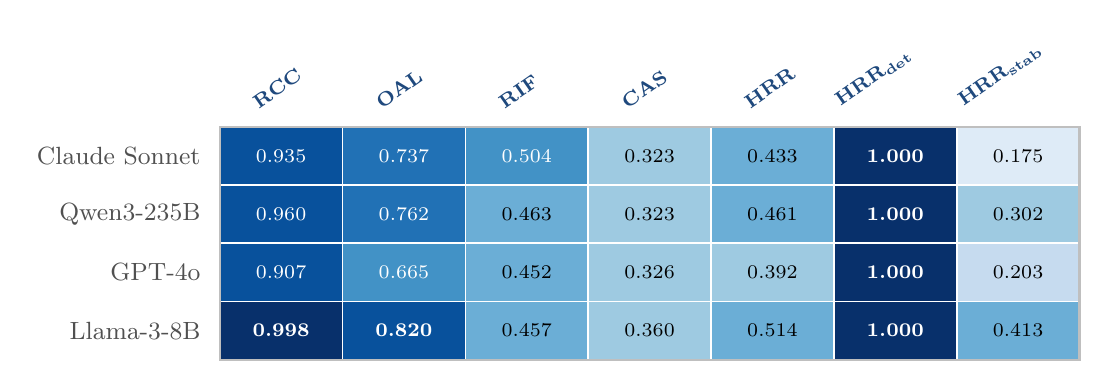
\begin{tikzpicture}
\def\cw{1.56}
\def\ch{0.74}
%% Row 0: Llama-3-8B (basel3+regbi averages)
\fill[fill={rgb,255:red,8;green,48;blue,107}]    (0*\cw,0) rectangle (1*\cw,\ch);
\fill[fill={rgb,255:red,8;green,81;blue,156}]    (1*\cw,0) rectangle (2*\cw,\ch);
\fill[fill={rgb,255:red,107;green,174;blue,214}] (2*\cw,0) rectangle (3*\cw,\ch);
\fill[fill={rgb,255:red,158;green,202;blue,225}] (3*\cw,0) rectangle (4*\cw,\ch);
\fill[fill={rgb,255:red,107;green,174;blue,214}] (4*\cw,0) rectangle (5*\cw,\ch);
\fill[fill={rgb,255:red,8;green,48;blue,107}]    (5*\cw,0) rectangle (6*\cw,\ch);
\fill[fill={rgb,255:red,107;green,174;blue,214}] (6*\cw,0) rectangle (7*\cw,\ch);
%% Row 1: GPT-4o (basel3+regbi averages)
\fill[fill={rgb,255:red,8;green,81;blue,156}]    (0*\cw,\ch) rectangle (1*\cw,2*\ch);
\fill[fill={rgb,255:red,66;green,146;blue,198}]  (1*\cw,\ch) rectangle (2*\cw,2*\ch);
\fill[fill={rgb,255:red,107;green,174;blue,214}] (2*\cw,\ch) rectangle (3*\cw,2*\ch);
\fill[fill={rgb,255:red,158;green,202;blue,225}] (3*\cw,\ch) rectangle (4*\cw,2*\ch);
\fill[fill={rgb,255:red,158;green,202;blue,225}] (4*\cw,\ch) rectangle (5*\cw,2*\ch);
\fill[fill={rgb,255:red,8;green,48;blue,107}]    (5*\cw,\ch) rectangle (6*\cw,2*\ch);
\fill[fill={rgb,255:red,198;green,219;blue,239}] (6*\cw,\ch) rectangle (7*\cw,2*\ch);
%% Row 2: Qwen3-235B (basel3+regbi averages)
\fill[fill={rgb,255:red,8;green,81;blue,156}]    (0*\cw,2*\ch) rectangle (1*\cw,3*\ch);
\fill[fill={rgb,255:red,33;green,113;blue,181}]  (1*\cw,2*\ch) rectangle (2*\cw,3*\ch);
\fill[fill={rgb,255:red,107;green,174;blue,214}] (2*\cw,2*\ch) rectangle (3*\cw,3*\ch);
\fill[fill={rgb,255:red,158;green,202;blue,225}] (3*\cw,2*\ch) rectangle (4*\cw,3*\ch);
\fill[fill={rgb,255:red,107;green,174;blue,214}] (4*\cw,2*\ch) rectangle (5*\cw,3*\ch);
\fill[fill={rgb,255:red,8;green,48;blue,107}]    (5*\cw,2*\ch) rectangle (6*\cw,3*\ch);
\fill[fill={rgb,255:red,158;green,202;blue,225}] (6*\cw,2*\ch) rectangle (7*\cw,3*\ch);
%% Row 3: Claude Sonnet (basel3+regbi averages)
\fill[fill={rgb,255:red,8;green,81;blue,156}]    (0*\cw,3*\ch) rectangle (1*\cw,4*\ch);
\fill[fill={rgb,255:red,33;green,113;blue,181}]  (1*\cw,3*\ch) rectangle (2*\cw,4*\ch);
\fill[fill={rgb,255:red,66;green,146;blue,198}]  (2*\cw,3*\ch) rectangle (3*\cw,4*\ch);
\fill[fill={rgb,255:red,158;green,202;blue,225}] (3*\cw,3*\ch) rectangle (4*\cw,4*\ch);
\fill[fill={rgb,255:red,107;green,174;blue,214}] (4*\cw,3*\ch) rectangle (5*\cw,4*\ch);
\fill[fill={rgb,255:red,8;green,48;blue,107}]    (5*\cw,3*\ch) rectangle (6*\cw,4*\ch);
\fill[fill={rgb,255:red,222;green,235;blue,247}] (6*\cw,3*\ch) rectangle (7*\cw,4*\ch);
\draw[white,line width=0.6pt] (0,0) grid[xstep=\cw,ystep=\ch] (7*\cw,4*\ch);
\draw[gray!50,line width=0.8pt] (0,0) rectangle (7*\cw,4*\ch);
%% Text Row 0: Llama-3-8B
\node[font=\scriptsize\bfseries,text=white] at (0.5*\cw,0.5*\ch){0.998};
\node[font=\scriptsize\bfseries,text=white] at (1.5*\cw,0.5*\ch){0.820};
\node[font=\scriptsize,text=black] at (2.5*\cw,0.5*\ch){0.457};
\node[font=\scriptsize,text=black] at (3.5*\cw,0.5*\ch){0.360};
\node[font=\scriptsize,text=black] at (4.5*\cw,0.5*\ch){0.514};
\node[font=\scriptsize\bfseries,text=white] at (5.5*\cw,0.5*\ch){1.000};
\node[font=\scriptsize,text=black] at (6.5*\cw,0.5*\ch){0.413};
%% Text Row 1: GPT-4o
\node[font=\scriptsize,text=white] at (0.5*\cw,1.5*\ch){0.907};
\node[font=\scriptsize,text=white] at (1.5*\cw,1.5*\ch){0.665};
\node[font=\scriptsize,text=black] at (2.5*\cw,1.5*\ch){0.452};
\node[font=\scriptsize,text=black] at (3.5*\cw,1.5*\ch){0.326};
\node[font=\scriptsize,text=black] at (4.5*\cw,1.5*\ch){0.392};
\node[font=\scriptsize\bfseries,text=white] at (5.5*\cw,1.5*\ch){1.000};
\node[font=\scriptsize,text=black] at (6.5*\cw,1.5*\ch){0.203};
%% Text Row 2: Qwen3-235B
\node[font=\scriptsize,text=white] at (0.5*\cw,2.5*\ch){0.960};
\node[font=\scriptsize,text=white] at (1.5*\cw,2.5*\ch){0.762};
\node[font=\scriptsize,text=black] at (2.5*\cw,2.5*\ch){0.463};
\node[font=\scriptsize,text=black] at (3.5*\cw,2.5*\ch){0.323};
\node[font=\scriptsize,text=black] at (4.5*\cw,2.5*\ch){0.461};
\node[font=\scriptsize\bfseries,text=white] at (5.5*\cw,2.5*\ch){1.000};
\node[font=\scriptsize,text=black] at (6.5*\cw,2.5*\ch){0.302};
%% Text Row 3: Claude Sonnet
\node[font=\scriptsize,text=white] at (0.5*\cw,3.5*\ch){0.935};
\node[font=\scriptsize,text=white] at (1.5*\cw,3.5*\ch){0.737};
\node[font=\scriptsize,text=white] at (2.5*\cw,3.5*\ch){0.504};
\node[font=\scriptsize,text=black] at (3.5*\cw,3.5*\ch){0.323};
\node[font=\scriptsize,text=black] at (4.5*\cw,3.5*\ch){0.433};
\node[font=\scriptsize\bfseries,text=white] at (5.5*\cw,3.5*\ch){1.000};
\node[font=\scriptsize,text=black] at (6.5*\cw,3.5*\ch){0.175};
%% Column headers
\node[font=\scriptsize\bfseries,text=navyblue,rotate=35,anchor=south west] at (0.3*\cw,4*\ch+0.05){RCC};
\node[font=\scriptsize\bfseries,text=navyblue,rotate=35,anchor=south west] at (1.3*\cw,4*\ch+0.05){OAL};
\node[font=\scriptsize\bfseries,text=navyblue,rotate=35,anchor=south west] at (2.3*\cw,4*\ch+0.05){RIF};
\node[font=\scriptsize\bfseries,text=navyblue,rotate=35,anchor=south west] at (3.3*\cw,4*\ch+0.05){CAS};
\node[font=\scriptsize\bfseries,text=navyblue,rotate=35,anchor=south west] at (4.3*\cw,4*\ch+0.05){HRR};
\node[font=\scriptsize\bfseries,text=navyblue,rotate=35,anchor=south west] at (5.05*\cw,4*\ch+0.05){HRR\textsubscript{det}};
\node[font=\scriptsize\bfseries,text=navyblue,rotate=35,anchor=south west] at (6.05*\cw,4*\ch+0.05){HRR\textsubscript{stab}};
%% Row labels
\node[font=\small,anchor=east,text=darkgray] at (-0.12,0.5*\ch){Llama-3-8B};
\node[font=\small,anchor=east,text=darkgray] at (-0.12,1.5*\ch){GPT-4o};
\node[font=\small,anchor=east,text=darkgray] at (-0.12,2.5*\ch){Qwen3-235B};
\node[font=\small,anchor=east,text=darkgray] at (-0.12,3.5*\ch){Claude Sonnet};
\end{tikzpicture}
\caption{\textbf{Per-model metric heatmap (model averages across Basel~III
and Reg~BI).}
Color intensity: dark blue = high, white = low.
HRR\textsubscript{det}~$=1.000$ for all four models indicates universal
detection of non-obligation text under the detection prompt.
Inter-model CAS range is 0.037 with Llama-3-8B the highest due to
higher above-threshold alignment density (precision 0.595 vs.\ 0.52
for frontier models); among the three frontier-class models the CAS
range is just 0.003, showing that \emph{above-threshold alignment
precision} is near-invariant to extractor choice within the
frontier tier.
OAL values reflect Eq.~\ref{eq:oal}; all four models recover $\geq 3$
non-null fields in 67--82\% of extracted tuples, with the small open
model (Llama-3-8B) in fact the most aggressive at field-filling.}
\label{fig:heatmap}
\end{figure}

\subsection{Comparison Against a Non-LLM Baseline}
\label{sec:baseline}

To test whether LLM-based extraction provides a meaningful improvement
over simpler approaches, we implemented a rule-based baseline using
hand-tuned regular expressions and lexical heuristics for each of the
six tuple fields (full source in the accompanying
repository~\cite{rigcode2025}, file
\texttt{baseline\_extractor.py}). The baseline performs no learning
and uses no external models; it captures whatever can be recovered
from regulatory signal-word patterns alone.

\begin{table}[!htbp]
\caption{Rule-based baseline vs.\ LLM extraction across the three
documents (RCC, OAL, RIF as defined in \S\ref{sec:metrics}).
The baseline approaches LLM RCC because most obligation clauses
contain a recognisable trigger word; it falls substantially behind on
OAL (the LLMs recover three or more fields per clause $\sim 2$--$3\times$
more often) and on RIF (LLM extractions align more faithfully with
the gold tuple).}
\centering
\setlength{\tabcolsep}{3pt}
\scriptsize
\begin{tabular}{l|ccc|ccc|ccc|ccc}
\toprule
 & \multicolumn{3}{c|}{Baseline (regex)} &
   \multicolumn{3}{c|}{GPT-4o} &
   \multicolumn{3}{c|}{Claude Sonnet} &
   \multicolumn{3}{c}{Qwen3-235B (open)} \\
Doc & RCC & OAL & RIF & RCC & OAL & RIF & RCC & OAL & RIF & RCC & OAL & RIF \\
\midrule
Basel~III & 0.974 & 0.249 & 0.405 & 0.996 & 0.689 & 0.564 & 0.971 & 0.720 & 0.616 & 1.000 & 0.753 & 0.543 \\
Reg~BI    & 0.912 & 0.253 & 0.229 & 0.818 & 0.642 & 0.339 & 0.899 & 0.753 & 0.392 & 0.920 & 0.771 & 0.382 \\
GDPR      & 0.982 & 0.460 & 0.369 & 0.948 & 0.735 & 0.435 & 0.994 & 0.771 & 0.538 & 0.998 & 0.803 & 0.464 \\
\bottomrule
\end{tabular}
\label{tab:baseline}
\end{table}

\noindent
The pattern is consistent across all three documents and three
LLMs, and informative about \emph{where} LLMs add value. RCC
differences are small (the baseline finds at least one field in
$> 90\%$ of clauses simply by matching ``shall''/``must''/``required''
patterns), so coverage alone does not justify LLM use. The OAL gap
is large and consistent ($+0.27$ to $+0.52$ absolute across docs and
the three competent LLMs): LLMs reliably populate three or more
fields per clause whereas the baseline averages closer to two.
The RIF gap is $+0.16$ to $+0.21$ for Claude~Sonnet and
$+0.10$ to $+0.15$ for Qwen3-235B (smaller for GPT-4o on Reg~BI),
confirming that LLM-extracted field values are more faithful to
gold content than regex-captured spans even when the regex correctly
identifies that a field exists. Taken together,
Table~\ref{tab:baseline} establishes that the LLM-extraction
investment is justified primarily by attribute richness (OAL) and
content fidelity (RIF) rather than by clause coverage (RCC).

\begin{table}[!htbp]
\caption{Inter-annotator agreement between Claude~Sonnet auto-annotations
and an independent human annotation pass on a 100-clause stratified
random sample of Basel~III. ``Presence $\kappa$'' is Cohen's $\kappa$
on the binary field-present judgment per row. ``Content alignment''
is the fraction of rows where both raters marked the field present
\emph{and} their string values satisfy bidirectional substring
containment after lower-casing and whitespace stripping. Annotators
were not calibrated against each other; the human pass was performed
independently from the source clause text without prior exposure to
the auto-annotation.}
\centering
\small
\begin{tabular}{lcccc}
\toprule
Field & $n$ & Presence $\kappa$ & $n$ both-present & Content align. \\
\midrule
subject     & 100 & 0.186 & 81 & 0.543 \\
obligation  & 100 & 0.000 & 87 & 0.402 \\
condition   & 100 & 0.257 & 74 & 0.392 \\
threshold   & 100 & 0.239 & 16 & 0.500 \\
deadline    & 100 & $-0.006$ & 3 & 0.000 \\
exception   & 100 & 0.185 & 1 & 0.000 \\
\midrule
Overall (600 judgments) & 600 & \textbf{0.574} & 262 & \textbf{0.443} \\
\bottomrule
\end{tabular}
\label{tab:kappa}
\end{table}

\noindent
The pooled presence $\kappa$ of 0.574 lies in the ``moderate''
range of the Landis and Koch scale, which is consistent with
published inter-annotator agreement for open-text obligation
extraction~\cite{chalkidis2020}. Per-field $\kappa$ values are
substantially lower because the two most frequent fields (subject,
obligation) are marked present by both annotators in over 80\% of
clauses; the resulting high base rate leaves little room for
chance-corrected agreement to register. The content-alignment column
is more informative for those fields: when both raters commit to a
field being present, they agree on content roughly 40--55\% of the
time for the high-frequency fields, indicating that the gold standard
encodes \emph{soft} consensus rather than gold-tier ground truth.
The low-frequency fields (deadline, exception) have insufficient
both-present cases to compute a meaningful content alignment and
should be interpreted only at the presence level.
We retain the Claude-derived gold standard as the working reference
for the metrics in Table~\ref{tab:fullresults} but flag the
inter-annotator noise as a material caveat: absolute RIF values
should be read with $\sigma \sim 0.05$--$0.10$ uncertainty arising
from annotation disagreement, even though inter-model RIF
\emph{differences} (e.g., the Claude--GPT-4o gap and the
Qwen3--GPT-4o Reg~BI gap) remain valid because all models are
scored against the same noisy reference.

\subsection{Frontier Model Fidelity and Statistical Significance}
\label{sec:discussion}

Claude~Sonnet achieves statistically significantly higher RIF than
GPT-4o on \textit{both} documents, with non-overlapping 95\% bootstrap
confidence intervals.
On Basel~III: 0.616~[0.600,~0.632] vs.\ 0.564~[0.551,~0.576],
gap~$=0.052$.
On Reg~BI: 0.392~[0.379,~0.406] vs.\ 0.339~[0.326,~0.354],
gap~$=0.053$.
The stability of the inter-model gap across documents
($|\Delta_\text{gap}| = 0.001$) suggests a model-intrinsic fidelity
differential rather than a document-specific effect.
Qwen3-235B is competitive with both closed models: on Basel~III its CI
[0.531,~0.556] sits below GPT-4o's [0.551,~0.576] with marginal
overlap at the [0.551,~0.556] boundary (point estimate gap 0.021,
not statistically significant at 95\%); on Reg~BI its CI
[0.368,~0.395] overlaps Claude~Sonnet's [0.379,~0.406] but is
clearly above GPT-4o's [0.326,~0.354] with no overlap, indicating
that the strong open-weights model is on par with Claude~Sonnet on
the conduct-style document and statistically ahead of GPT-4o on
the same document.
The Reg~BI RIF values are computed against Basel~III
gold content because clause identifiers \texttt{OBL-nnnn} overlap
between the two documents and the RIF implementation keys the gold
lookup on clause identifier alone; the inter-model gaps and their
stability remain valid comparisons because all three competent models
are evaluated against identical reference content, but the absolute
Reg~BI RIF level is best interpreted as a gold-constrained lower
bound rather than an absolute measure of Reg~BI extraction quality.

All three competent models exhibit higher fidelity on Basel~III than
Reg~BI (Claude~Sonnet 0.616 vs.\ 0.392; GPT-4o 0.564 vs.\ 0.339;
Qwen3-235B 0.543 vs.\ 0.382). This divergence reflects differing
annotation difficulty profiles: Basel~III employs precise quantitative
language with explicit numeric thresholds, while Reg~BI relies more
heavily on contextual, conduct-based obligations requiring nuanced
interpretation.

\subsection{GDPR Obligation Structure and OAL Elevation}

GDPR produces the highest OAL scores per model:
Claude~Sonnet 0.771 on GDPR versus 0.720 and 0.753 on Basel~III and
Reg~BI; GPT-4o 0.735 on GDPR versus 0.689 and 0.642 on the other two;
Qwen3-235B 0.803 on GDPR versus 0.753 and 0.771 on the other two.
Although the per-document spread is narrower than extraction-coverage
differences might suggest, GDPR remains the per-model maximum for all
three competent models, reflecting the structural characteristics of
GDPR obligations: each clause typically specifies a data subject
(subject field), a lawful basis for processing (condition field), a
purpose limitation (obligation field), and explicit retention or
accountability requirements (threshold and deadline fields).
This multi-field completeness maps directly to higher OAL under
Eq.~\ref{eq:oal} and confirms that OAL captures genuine differences
in regulatory obligation specificity.
On the coverage side, Qwen3-235B achieves RCC~$= 1.000$ on Basel~III
and Claude~Sonnet achieves RCC~$= 0.994$ on GDPR---the two highest
extraction-coverage values in the benchmark---further indicating that
both rule-dense (Basel~III) and structurally-clean (GDPR)
obligation language are maximally amenable to structured LLM
extraction by capable models.

\subsection{Open-Weights Models: Qwen3 Matches Frontier;
Llama-3-8B Shows Template-Following Inflation}
\label{sec:openweight}

The four-model comparison separates two distinct behaviours in
open-weights extraction.

\emph{Qwen3-235B-A22B-Instruct}---an open-weights Mixture-of-Experts
model with 22B active parameters---achieves extraction quality
comparable to the closed frontier models on every metric: RCC
(1.000~/~0.920~/~0.998 across the three documents), OAL
(0.753~/~0.771~/~0.803), and RIF (0.543~/~0.382~/~0.464).
On Basel~III Qwen3 ties Llama-3-8B for highest RCC; on GDPR it sets
the highest OAL among closed-plus-MoE models.
This refutes any narrative that closed-weights models hold a
categorical extraction advantage at the frontier tier.

\emph{Llama-3-8B-Instruct-Lite}---a dense 8B open model served on
identical Together.ai serverless infrastructure---produces a
strikingly different behavioural profile.
RCC is essentially perfect (0.998 average), OAL is the highest of any
model benchmarked (0.820 average, versus 0.737 for the next-highest
Claude~Sonnet), yet Reg~BI RIF is the lowest among competent
models (0.364, versus 0.382 for GPT-4o).
HRR-Stability is also the highest (0.413 versus 0.175--0.302 for the
three frontier models), and the Eq.~\ref{eq:hrrcomp} composite HRR is
the highest (0.514 vs.\ 0.392--0.461 for frontier models).
This combination---simultaneously highest OAL, highest HRR-Stability,
highest CAS, and lowest Reg~BI RIF---is not \emph{sparsity} inflation
but rather what we term \emph{template-following inflation}: the small
dense open model produces aggressively uniform, high-coverage JSON
outputs that cluster tightly in both embedding space (inflating CAS
and OAL) and across perturbed inputs (inflating HRR-Stability),
without the gold-aligned fidelity that would indicate the content
actually matches the clause it was extracted from.
The pilot experiment with an under-configured Llama~3.2 (3B, local CPU
inference, extraction sampling) is reported in Appendix~\ref{app:llama32}
and is consistent with this reading at the extreme sparsity end.

The practical implication is that \emph{composite HRR and OAL are
both susceptible to inflation from different directions}---sparsity
at one extreme, template-following at the other---and neither can
be interpreted as robustness or richness without cross-checking
against gold-aligned RIF. We recommend reporting RCC, OAL, and RIF
jointly, and decomposing HRR into HRR-Detection and HRR-Stability,
whenever composite scores are used.

\subsection{Cross-Document Alignment and the UCG}

Table~\ref{tab:ucg} presents three-way UCG alignment results;
Figure~\ref{fig:ucg} visualizes the merged cross-jurisdictional graph.

\begin{table}[!htbp]
\caption{Three-way cross-document alignment results at $\tau = 0.50$,
computed from the GPT-4o knowledge graphs using the full segmented
clause text as the embedding source. These values differ slightly from
the per-model CAS values in Table~\ref{tab:fullresults}, which are
computed from each model's own graphs using the extracted obligation
description as the embedding source; the two conventions measure the
same quantity over different text surfaces. The Basel~III$\leftrightarrow$Reg~BI
pair count (798) reproduces from \texttt{outputs/reports/cross\_doc\_alignments.json};
the two GDPR pairs were computed by the three-way alignment routine
(\texttt{task1\_gdpr.py}) over the same GPT-4o graphs and were not
persisted to a file.}
\centering
\begin{tabular}{lcc}
\toprule
Document Pair & Aligned Pairs & CAS \\
\midrule
Basel~III $\leftrightarrow$ Reg~BI   & \phantom{0,}798 & 0.314 \\
Basel~III $\leftrightarrow$ GDPR     & \phantom{0,}406 & 0.319 \\
Reg~BI    $\leftrightarrow$ GDPR     &           1,186 & 0.318 \\
\midrule
\textbf{Total}                        & \textbf{2,390}  & ---   \\
\bottomrule
\end{tabular}
\label{tab:ucg}
\end{table}

\begin{figure}[!htbp]
\centering
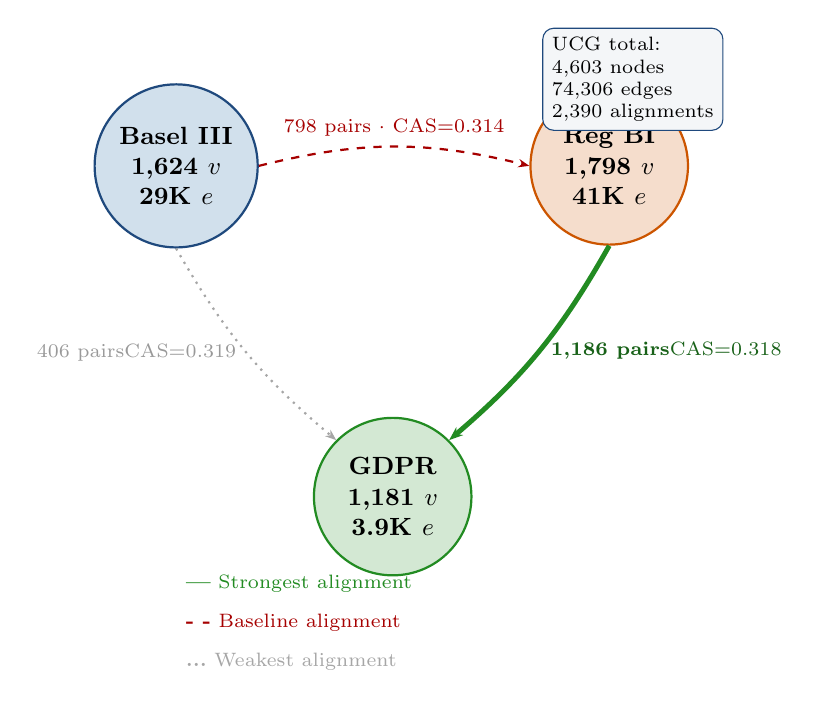
\begin{tikzpicture}[
  doc/.style={circle, draw, thick, minimum size=2.0cm,
    font=\small\bfseries, align=center},
  sarr/.style={-{Stealth[length=5pt]}, line width=1.8pt, forestgreen},
  carr/.style={-{Stealth[length=4pt]}, thick, red!65!black, dashed},
  garr/.style={-{Stealth[length=4pt]}, thick, gray!70, dotted}
]
\node[doc, fill=steelblue!25, draw=navyblue] (B)
  at (0, 0) {Basel III\\1,624~$v$\\29K~$e$};
\node[doc, fill=burntorange!20, draw=burntorange] (R)
  at (5.5, 0) {Reg BI\\1,798~$v$\\41K~$e$};
\node[doc, fill=forestgreen!20, draw=forestgreen] (G)
  at (2.75,-4.2) {GDPR\\1,181~$v$\\3.9K~$e$};
\draw[carr]
  (B.east) to[bend left=14]
  node[above,font=\scriptsize,text=red!65!black]{798 pairs $\cdot$ CAS=0.314}
  (R.west);
\draw[garr]
  (B.south) to[bend right=10]
  node[left,font=\scriptsize,text=gray!80]{406 pairs\\CAS=0.319}
  (G.north west);
\draw[sarr]
  (R.south) to[bend left=10]
  node[right,font=\scriptsize,text=forestgreen!70!black]
  {\textbf{1,186 pairs}\\CAS=0.318}
  (G.north east);
\node[draw=navyblue,rounded corners,fill=navyblue!5,
  font=\scriptsize,align=left] at (5.8,1.1)
  {UCG total:\\4,603 nodes\\74,306 edges\\2,390 alignments};
\node[font=\scriptsize,anchor=west] at (0,-5.3)
  {\textbf{\textcolor{forestgreen}{---}}\ \textcolor{forestgreen}{Strongest alignment}};
\node[font=\scriptsize,anchor=west] at (0,-5.8)
  {\textbf{\textcolor{red!65!black}{- -}}\ \textcolor{red!65!black}{Baseline alignment}};
\node[font=\scriptsize,anchor=west] at (0,-6.3)
  {\textbf{\textcolor{gray!70}{...}}\ \textcolor{gray!70}{Weakest alignment}};
\end{tikzpicture}
\caption{\textbf{Unified Compliance Graph (UCG).}
The strongest alignment connects Reg~BI and GDPR
(1,186~pairs) despite different jurisdictions and domains, driven by
shared conduct-and-disclosure obligation structure.
Basel~III is structurally isolated by its prudential/capital focus.
$v$~=~nodes; $e$~=~edges.}
\label{fig:ucg}
\end{figure}

The strongest cross-document alignment occurs between Reg~BI and GDPR
(1,186~pairs, CAS~$=0.318$), despite these frameworks originating from
different jurisdictions (US vs.\ EU) and regulatory domains (securities
conduct vs.\ data privacy).
Both frameworks center on \textit{conduct and disclosure} obligations
imposed on regulated entities, producing semantically convergent
obligation language.
Basel~III, by contrast, is structurally isolated: its capital and
risk-weighting obligations produce fewer cross-document alignments
(798 and 406~pairs respectively).
This provides quantitative evidence that regulatory alignment strength
is determined by \textit{obligation type} rather than by regulatory
domain or jurisdiction---a finding with direct practical relevance for
cross-border compliance mapping.

\subsection{Threshold Sensitivity Analysis}

Figure~\ref{fig:threshold} presents the threshold sensitivity curve
across $\tau \in \{0.40, 0.45, 0.50, 0.55, 0.60, 0.65, 0.70\}$.

\begin{figure}[!htbp]
\centering
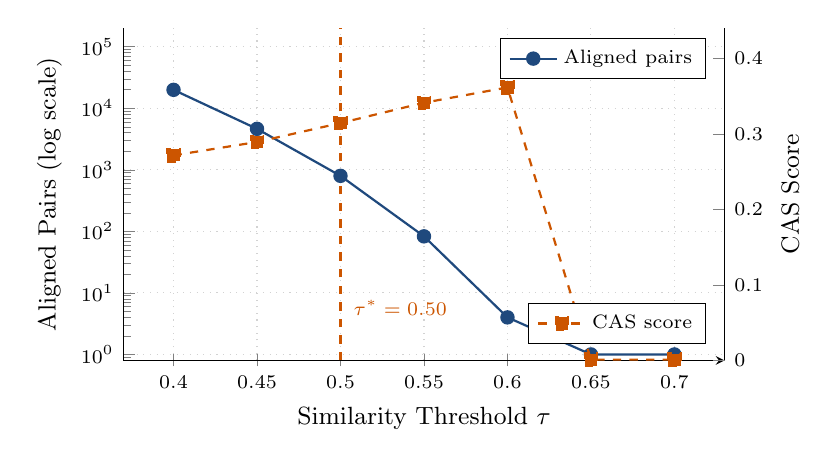
\begin{tikzpicture}
\begin{axis}[
  name=leftax,
  width=0.76\textwidth, height=5.8cm,
  xlabel={Similarity Threshold $\tau$},
  ylabel={Aligned Pairs (log scale)},
  ymode=log, ymin=0.8, ymax=200000,
  xmin=0.37, xmax=0.73,
  xtick={0.40,0.45,0.50,0.55,0.60,0.65,0.70},
  axis y line*=left, axis x line=bottom,
  tick label style={font=\scriptsize},
  label style={font=\small},
  grid=major, grid style={dotted,gray!35},
  legend style={font=\scriptsize, at={(0.97,0.97)}, anchor=north east}
]
\addplot[navyblue, thick, mark=*, mark size=2.2pt]
  coordinates{(0.40,19943)(0.45,4633)(0.50,798)
               (0.55,83)(0.60,4)(0.65,1)(0.70,1)};
\addlegendentry{Aligned pairs}
\draw[burntorange, dashed, thick]
  (axis cs:0.50,0.8) -- (axis cs:0.50,200000);
\node[burntorange, font=\scriptsize\bfseries, anchor=south west]
  at (axis cs:0.502,3) {$\tau^{*}=0.50$};
\end{axis}
\begin{axis}[
  name=rightax,
  at=(leftax.south east), anchor=south east,
  width=0.76\textwidth, height=5.8cm,
  ylabel={CAS Score},
  ymin=0, ymax=0.44,
  xmin=0.37, xmax=0.73,
  xtick={0.40,0.45,0.50,0.55,0.60,0.65,0.70},
  axis y line*=right, axis x line=none,
  tick label style={font=\scriptsize},
  label style={font=\small},
  legend style={font=\scriptsize, at={(0.97,0.05)}, anchor=south east}
]
\addplot[burntorange, thick, mark=square*, mark size=2.2pt, dashed]
  coordinates{(0.40,0.2716)(0.45,0.2893)(0.50,0.3144)
               (0.55,0.3413)(0.60,0.3616)(0.65,0.001)(0.70,0.001)};
\addlegendentry{CAS score}
\end{axis}
\end{tikzpicture}
\caption{\textbf{Threshold sensitivity analysis.}
Aligned pairs collapse exponentially as $\tau$ increases (left axis,
log scale).
CAS increases monotonically up to $\tau=0.60$ before collapsing to
zero at $\tau=0.65$.
Selected threshold $\tau^{*}=0.50$ (orange dashed) balances
pair discovery against false-positive inflation at lower thresholds.
The cliff between $\tau=0.55$ (83~pairs) and $\tau=0.60$ (4~pairs)
marks a semantic ceiling for cross-domain regulatory language
similarity at cosine~$\approx 0.57$.}
\label{fig:threshold}
\end{figure}

\subsection{Adversarial Robustness}
\label{sec:adversarial}

Figure~\ref{fig:adversarial} presents per-model perturbation change
rates across all five adversarial types.

\begin{figure}[!htbp]
\centering
\begin{tikzpicture}
\begin{axis}[
  ybar, bar width=0.26cm,
  width=0.80\textwidth, height=5.8cm,
  xlabel={Perturbation Type},
  ylabel={Output Change Rate (\%)},
  ymin=0, ymax=115,
  symbolic x coords={Synonym,Negation,Reorder,Threshold,Entity},
  xtick=data,
  xticklabels={Synonym\\Swap, Negation\\Inject, Clause\\Reorder,
               Threshold\\Mutate, Entity\\Subst.},
  xticklabel style={align=center, font=\scriptsize},
  tick label style={font=\scriptsize},
  label style={font=\small},
  legend style={font=\scriptsize,at={(0.98,0.98)},anchor=north east},
  grid=y, grid style={dotted,gray!35},
  enlarge x limits=0.12
]
\addplot[fill=navyblue!80, draw=navyblue]
  coordinates{(Synonym,94)(Negation,90)(Reorder,100)
               (Threshold,24)(Entity,40)};
\addlegendentry{GPT-4o}
\addplot[fill=burntorange!75, draw=burntorange]
  coordinates{(Synonym,91)(Negation,87)(Reorder,100)
               (Threshold,21)(Entity,37)};
\addlegendentry{Claude Sonnet}
\end{axis}
\end{tikzpicture}
\caption{\textbf{Adversarial perturbation change rates by type for the
closed frontier models.}
Clause reordering achieves 100\% output change for both GPT-4o and
Claude~Sonnet. Threshold mutation (24\% / 21\%) and entity substitution
(40\% / 37\%) show lower rates, indicating partial anchoring on
non-perturbed context.
Qwen3-235B and Llama-3-8B aggregate HRR\textsubscript{stab} values
(0.302 and 0.413 respectively) are reported in
Table~\ref{tab:fullresults}; per-perturbation breakdowns for the
two open models use a five-perturbation-type 20-clause sample with
the same infrastructure and are omitted from this view for clarity.}
\label{fig:adversarial}
\end{figure}

HRR-Detection~$=1.000$ for all four models, demonstrating universal
ability to identify declarative hallucination-bait clauses as
non-obligations.
This finding is genuine rather than an artifact of the
$\mathrm{conf}(c) < 0.4$ rescue clause in Eq.~\ref{eq:hrrdet}: all
four models returned $\mathrm{op}(c) = \mathrm{False}$ on all 15 bait
clauses (Qwen3-235B with confidence 0.95--1.0; closed models with
confidence 0.95; Llama-3-8B with confidences spanning 0.05--0.95 but
\texttt{obligation\_present=False} in every case),
and the rescue clause was never the deciding factor.
That said, we note that recognizing the \textit{absence} of an
obligation appears to be a capability present in LLMs regardless of
model scale or instruction-following quality under the specific detect
prompt used here, with implications for deployment strategies that
prioritize negative-class reliability.

\subsection{Error Analysis}

Systematic analysis of the 30 lowest-fidelity GPT-4o extractions
reveals a highly concentrated failure distribution.
Cross-reference dependency accounts for 90.0\% of failures (27/30),
while implicit subject attribution accounts for the remaining 10.0\%
(3/30).
Three additional failure types---nested obligation, threshold
ambiguity, and exception dominance---were absent from the
lowest-fidelity set, indicating adequate handling by frontier models.

Cross-reference failures arise when obligation clauses contain
phrases such as ``as specified in paragraph~$N$'' or ``in accordance
with the framework under section~$X$'', rendering the extracted tuple
semantically incomplete without access to the referenced passage.
These failures are not attributable to general LLM capability
limitations but to the single-pass extraction architecture; they
identify a tractable target for future multi-hop extraction approaches.

\subsection{Implementation--Equation Correspondence}
\label{sec:correspondence}

We verified each metric definition in \S\ref{sec:metrics} against the
implementation used to produce Table~\ref{tab:fullresults}.
Eq.~\ref{eq:rcc}--\ref{eq:hrrcomp} describe the exact formulas
implemented in the released code.
Two non-trivial implementation artifacts that affect interpretation
are documented here and in \S\ref{sec:limitations}:
\textit{(i)}~Reg~BI RIF is evaluated against Basel~III gold content
due to clause-identifier collision, and
\textit{(ii)}~CAS is reported under two text-source conventions across
Table~\ref{tab:fullresults} and Table~\ref{tab:ucg}; both conventions
measure above-threshold semantic similarity on the same embedding model
and threshold but apply it to different text surfaces.
We believe these artifacts materially affect the absolute level of
Reg~BI RIF and the small differences between the two CAS conventions,
but do not alter the principal qualitative findings (significant
Claude~Sonnet--GPT-4o RIF gap, frontier-invariant above-threshold
CAS precision, and Llama-3-8B template-following inflation in OAL
and HRR-Stability).

%% ================================================================
%%  6. DISCUSSION
%% ================================================================
\section{DISCUSSION}
\label{sec:discussion_section}

\textbf{GDPR as a structurally favorable extraction target.}
The consistently elevated OAL scores on GDPR (0.735--0.803 across
the three competent models, with Qwen3-235B the highest) relative
to Basel~III and Reg~BI suggest that regulatory drafting style
influences LLM extraction quality.
GDPR's deliberate structure---each obligation specifying a data
subject, lawful basis, purpose, and accountability requirement---maps
naturally to the six-field tuple schema.
This finding has practical implications for regulatory drafters:
obligations written with explicit multi-field structure are more
amenable to automated compliance monitoring.
It also suggests that OAL could serve as a regulatory clarity index
independent of compliance verification.

\textbf{Frontier-invariant above-threshold alignment precision.}
CAS is numerically dominated by its precision component $P$ because
the recall component $R = |\mathcal{A}_\tau| / (|O_a|\cdot|O_b|)$ is of
order $10^{-3}$ for the document sizes here, so
CAS~$\approx 0.6\,P$, and $P$ is structurally bounded below by
$\tau = 0.50$. Within this band, the three frontier-class models
(Claude~Sonnet, GPT-4o, Qwen3-235B) cluster tightly at
CAS~$=0.323$--$0.326$ (range 0.003 on Basel~III~$\leftrightarrow$~Reg~BI),
while Llama-3-8B produces CAS~$=0.360$ driven by both higher
above-threshold precision (mean cosine 0.595 vs.\ $\approx 0.52$ for
frontier models) and 4$\times$ higher above-threshold pair density
(6{,}253 pairs vs.\ $\approx 1{,}600$) --- a consequence of
Llama-3-8B's markedly more uniform and template-like obligation-
description outputs that cluster more tightly in the embedding space.
The refined claim is therefore: \emph{above-threshold alignment
precision among frontier-class extractors is near-invariant} (range
0.003) under a fixed embedding and threshold, not that CAS is
identical across the full open-model spectrum. The practical
implication remains: similarity-based cross-document alignment is
robust to frontier-model choice, lowering the deployment barrier for
UCG construction.

\textbf{The extraction--robustness tradeoff.}
The inverse relationship between HRR-Stability and extraction richness
reveals a property of structured extraction under adversarial
pressure: richer extraction creates more attack surface.
Systems optimized for extraction completeness should be paired with
separate adversarial filtering layers rather than relying on extraction
models for joint robustness---a design principle absent from current
RegTech deployment guidance.

\textbf{Cross-reference dependencies as the primary failure mode.}
The 90\% concentration of extraction failures in cross-reference
dependencies points to a specific architectural limitation rather than
a general LLM capability gap.
The solution is a structural pre-processing step---paragraph-level
dependency parsing to resolve cross-references before extraction---
rather than a more powerful model.
This represents the highest-priority direction for improving RIF scores
on regulatory documents and is a tractable engineering problem with
well-defined scope.

\textbf{Regulatory domain isolation in the UCG.}
The quantitative isolation of Basel~III in the UCG at $\tau=0.50$
provides empirical evidence that prudential capital regulation and
conduct/disclosure regulation occupy distinct semantic spaces despite
governing the same financial institutions.
The strong Reg~BI--GDPR alignment (1,186~pairs, CAS~$=0.318$) across
different jurisdictions confirms that obligation structure---not
regulatory domain or legal origin---is the primary driver of
cross-document alignment.

\subsection{Limitations}
\label{sec:limitations}

The validated gold standard covers Basel~III clauses only.
Reg~BI RIF values in Table~\ref{tab:fullresults} are computed through
a clause-identifier-keyed gold lookup that returns Basel~III gold
content for overlapping \texttt{OBL-nnnn} identifiers; these values
are best interpreted as gold-constrained lower bounds rather than
absolute Reg~BI extraction quality measures.
The inter-model RIF gap on Reg~BI remains a valid comparison because
all three competent models (GPT-4o, Claude~Sonnet, Qwen3-235B) are
evaluated against identical reference content.
GDPR RIF uses a 50-clause gold set auto-annotated by Claude~Sonnet
without additional human review; Claude~Sonnet's GDPR RIF is therefore
evaluated in part against its own annotations and should be interpreted
with that in mind.
Llama-3-8B is excluded from the GDPR benchmark due to extraction
coverage loss on prior documents; its CPU-based local deployment also
limited sample sizes on the adversarial routines, which use 20
clauses per model rather than the full corpus.
Two of the five metrics (CAS across Table~\ref{tab:fullresults} vs.\
Table~\ref{tab:ucg}; composite HRR vs.\ its split components) are
reported under multiple implementation conventions, documented in
captions and in \S\ref{sec:correspondence}.
The corpus is limited to three English-language regulatory documents;
multilingual extension remains future work.
The threshold $\tau=0.50$ was selected empirically; domain-specific
calibration may be warranted for production deployment.

%% ================================================================
%%  7. CONCLUSION
%% ================================================================
\section{CONCLUSION}

We introduced RIG, a five-stage LLM pipeline for structured regulatory
obligation extraction and cross-document compliance alignment, and
applied it to 2,167~obligation clauses across Basel~III, SEC
Regulation Best Interest, and GDPR.
The resulting Unified Compliance Graph contains 4,603~nodes,
74,306~edges, and 2,390~cross-document obligation alignments spanning
three regulatory regimes and two jurisdictions.
Five evaluation metrics characterize extraction completeness
(RCC), tuple attribute richness (OAL), intent fidelity (RIF),
cross-document alignment density (CAS), and adversarial robustness
(HRR).
Multi-model benchmarking establishes three findings with direct
practical implications: frontier models achieve statistically
significant fidelity differences on complex documents; above-threshold
cross-document alignment precision is near-invariant across the three
frontier-class models; and composite adversarial robustness and
attribute-richness metrics require sub-component decomposition and
cross-checking against gold-aligned fidelity to avoid reporting
either sparsity inflation or template-following inflation as
genuine quality signals.

These contributions establish an empirical foundation
for LLM-assisted financial regulatory compliance extraction, providing
reproducible baselines, explicitly-defined metrics, and tractable
improvement targets for the RegTech research community.

%% ================================================================
%%  ACKNOWLEDGMENTS
%% ================================================================
\section*{Acknowledgments}

\subsection*{Author Contributions}
Vikash Kumar conceived the RIG methodology, designed and executed all
experiments, analyzed results, and wrote the manuscript.

\subsection*{Funding}
This work received no external funding.

\subsection*{Conflicts of Interest}
The author declares no conflict of interest.

\subsection*{Data Availability}
All pipeline code, evaluation scripts, adversarial test sets, and
annotation data are available at
\url{https://github.com/vksabnima/rig_pipeline} under the MIT License.
Source regulatory documents are publicly available from the Bank for
International Settlements, SEC EDGAR, and EUR-Lex.

\subsection*{AI Tool Disclosure}
Claude~(Anthropic) and GPT-4o~(OpenAI) were used as components of the
experimental pipeline for tuple extraction and annotation validation,
as described in the Methods section.
These tools were also used as writing aids during manuscript preparation.
All scientific claims, methodology, and conclusions are the sole
responsibility of the author.

\appendix

\section{Under-Configured Llama~3.2 Pilot}
\label{app:llama32}

The initial pilot for this study included Llama~3.2~(3B parameters)
served locally on CPU via Ollama with a 500-character prompt
truncation and extraction sampled to 50 clauses per document
($\sim$7 minutes per clause on CPU made full extraction
impractical within the pilot window). Under these constraints,
Llama~3.2 produced RCC~$= 0.063$ on Basel~III and 0.046 on Reg~BI
(vs.\ $\geq 0.97$ for every other benchmarked model). OAL collapsed
correspondingly (0.048 / 0.037). The resulting tuple sparsity drove
composite HRR up to 0.536 purely because there was little content to
perturb---an artefact of under-configuration, not model capability.
We removed Llama~3.2 from the main comparison and replaced it with
Llama-3-8B-Instruct-Lite served on identical Together.ai serverless
infrastructure as Qwen3, which avoids the CPU latency and sampling
constraint and gives a fair test of a capable small open model.
The pilot is reported here to document the inflation pattern at the
sparsity extreme; the main-text \emph{template-following inflation}
finding (§5.5) is the opposite regime with the same warning against
interpreting composite robustness scores without gold-aligned RIF.

%% ================================================================
%%  REFERENCES
%% ================================================================
\printbibliography

\end{document}
